Тестирование функций было проведено по стратегии черного ящика.
Под <<черным ящиком>> понимается объект исследования, внутреннее устройство которого неизвестно.
Черный ящик в кибернетике позволяет изучать поведение систем, то есть их реакций на разнообразные внешние воздействия и в то же время абстрагироваться от их внутреннего устройства.
Манипулируя только лишь со входами и выходами, можно проводить определенные исследования.

Сравнение содержимого документов, выполняемое в данном разделе, проводился с использованием утилиты GNU/diff~--- инструментального средства для построчного сравнения файлов.
diff является утилитой командной строки, обладающей следующим синтаксисом запуска:
\begin{lstlisting}
  diff [ ОПЦИИ  ] [ ФАЙЛЫ  ]
\end{lstlisting}

Среди опций особого внимания заслуживает опция \textbf{-s}: при совпадении файлов ее использование приведет к выводу соответствующего сообщения.

\subsection{Добавление и удаление элементов}
\textbf{Исходные данные:}

Пустой документ.\\

\textbf{Механизм тестирования:}
\begin{enumerate}
  \item Добавить в схему метку.
  \item Сохранить документ, изучить его содержимое.
  \item Добавить в схему два узла.
  \item Сохранить документ, изучить его содержимое.
  \item Добавить в схему связь.
  \item Сохранить документ, изучить его содержимое.
  \item Удалить созданные элементы.
  \item Сохранить документ, изучить его содержимое.
\end{enumerate}

\textbf{Результат:}
\begin{enumerate}
  \item Добавленная метка:
  \begin{lstlisting}[xleftmargin=0cm]
<!DOCTYPE SVE>
<document height="560" width="980">
 <label id="1400577527716" x="0" y="0" text="TEST"/>
</document>
  \end{lstlisting}
  \item Добавленные узлы:
  \begin{lstlisting}[xleftmargin=0cm]
<!DOCTYPE SVE>
<document height="560" width="980">
 <label id="1400577527716" x="0" y="0" text="TEST"/>
 <node id="1400577736807" x="110" plugin="not_gate" y="30"/>
 <node id="1400577743141" x="0" plugin="not_gate" y="30"/>
</document>
  \end{lstlisting}
  \item Добавленная связь:
  \begin{lstlisting}[xleftmargin=0cm]
<!DOCTYPE SVE>
<document height="560" width="980">
 <label id="1400577527716" x="0" y="0" text="TEST"/>
 <node id="1400577736807" x="110" plugin="not_gate" y="30"/>
 <node id="1400577743141" x="0" plugin="not_gate" y="30"/>
 <link last_id="1400577736807" last_connector="0" first_id="1400577743141" id="1400577974692" first_connector="0"/>
</document>
  \end{lstlisting}
  \item Удаление элементов:
  \begin{lstlisting}[xleftmargin=0cm]
<!DOCTYPE SVE>
<document height="560" width="980">
 <label id="1400577527716" x="0" y="0" text="TEST"/>
 <node id="1400577736807" x="110" plugin="not_gate" y="30"/>
 <node id="1400577743141" x="0" plugin="not_gate" y="30"/>
</document>

<!DOCTYPE SVE>
<document height="560" width="980">
 <label id="1400577527716" x="0" y="0" text="TEST"/>
 <node id="1400577736807" x="110" plugin="not_gate" y="30"/>
</document>

<!DOCTYPE SVE>
<document height="560" width="980">
 <label id="1400577527716" x="0" y="0" text="TEST"/>
</document>

<!DOCTYPE SVE>
<document height="560" width="980"/>
  \end{lstlisting}
\end{enumerate}

Как видно, XML-документ последовательно изменялся, наполняясь новыми узлами по мере добавления элементов.
Удаление элементов ведет к удалению узлов из XML-дерева документа.
Можно сделать вывод, что процессы добавления и удаления элементов протекали нормально и без ошибок.


\subsection{Изменение элементов}
\textbf{Исходные данные:}

Проверяемый документ:
\begin{lstlisting}
<!DOCTYPE SVE>
<document height="560" width="980">
 <label id="1400577527716" x="0" y="0" text="TEST"/>
 <node id="1400578932545" x="0" plugin="not_gate" y="30"/>
 <node id="1400578944621" x="140" plugin="and_gate" y="40"/>
 <link last_id="1400578944621" last_connector="0" first_id="1400578932545" id="1400578956357" first_connector="0"/>
</document>
\end{lstlisting}

\textbf{Механизм тестирования:}
\begin{enumerate}
  \item Изменить текст метки.
  \item Переместить один из узлов.
  \item Изменить соединение связи.
  \item Сохранить документ, сравнить его с исходным.
\end{enumerate}

\textbf{Результат:}

\begin{lstlisting}
diff 0.sve 0-change.sve
\end{lstlisting}

Выполнение указанной команды позволит выявить различия в файлах.

\begin{lstlisting}
3c3
<  <label id="1400577527716" x="0" y="0" text="TEST"/>
---
>  <label id="1400577527716" x="0" y="0" text="CHANGE"/>
5,6c5,6
<  <node id="1400578944621" x="140" plugin="and_gate" y="40"/>
<  <link last_id="1400578944621" last_connector="0" first_id="1400578932545" id="1400578956357" first_connector="0"/>
---
>  <node id="1400578944621" x="130" plugin="and_gate" y="150"/>
>  <link last_id="1400578944621" last_connector="1" first_id="1400578932545" id="1400578956357" first_connector="0"/
\end{lstlisting}

Из вывода видно, что файлы различаются тремя строками:
\begin{enumerate}
  \item Метка с текстом <<TEST>> теперь содержит текст <<CHANGE>>.
  \item Узел <<and\_gate>>, ранее имевший координаты (140; 40) теперь имеет координаты (130; 150).
  \item last\_connector связи сменился с <<0>> на <<1>>.
\end{enumerate}

Указанные изменения в документе отразили произошедшие в документе правки, следовательно, процесс изменения элементов работал корректно.

\subsection{Сохранение и загрузка файлов}
\textbf{Исходные данные:}
\begin{figure}[H]
  \centering
  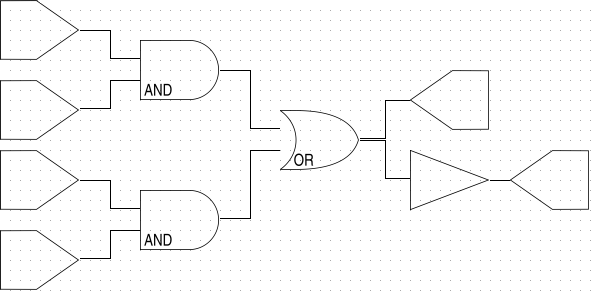
\includegraphics[width=0.6\textwidth]{gui/test/source.png}
  \caption{Проверяемая схема}
  \label{fig:source-test-scheme}
\end{figure}

\textbf{Механизм тестирования:}
\begin{enumerate}
  \item Сохранить схему.
  \item Открыть сохраненный файл.
  \item Сравнить внешний вид схемы с рисунком \ref{fig:source-test-scheme}.
  \item Сохранить схему повторно под другим именем.
  \item Сравнить полученные в результате файлы.
\end{enumerate}

\textbf{Результат:}
\begin{figure}[H]
  \centering
  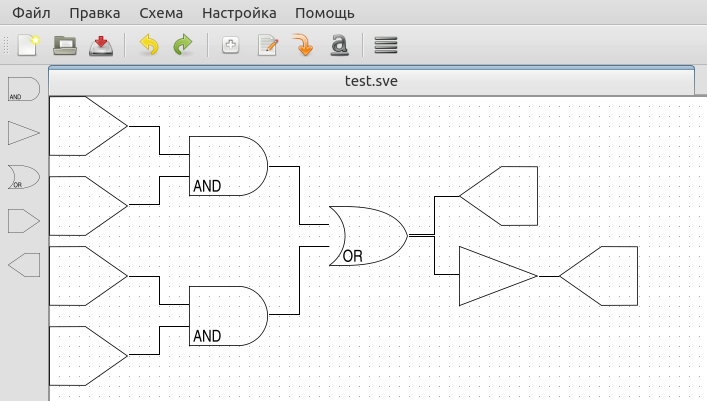
\includegraphics[width=0.7\textwidth]{gui/test/load-res.png}
  \caption{Загруженная схема}
  \label{fig:load-test-scheme}
\end{figure}

\begin{lstlisting}
diff -s test1.sve test2.sve
\end{lstlisting}

Выполнение указанной команды позволит определить, одинаковы ли файлы.
\begin{lstlisting}
Files test1.sve and test2.sve are identical
\end{lstlisting}

Визуальное изучение схемы и результат построчного сравнения файлов показали, что они идентичны.
Значит, процесс загрузки файлов протекал корректно, сохраняя структуру и содержимое документа.

\subsection{История изменений}
\textbf{Исходные данные:}

Пустой документ.\\

\textbf{Механизм тестирования:}
\begin{enumerate}
  \item Внести в документ изменение и сохранить документ (1).
  \item Внести в документ изменение и сохранить документ (1-change).
  \item Отменить изменение в документе.
  \item Сохранить его под новым именем (2).
  \item Сравнить внешний вид схем до внесения и после отмены изменения.
  \item Сравнить документы (1) и (2).
\end{enumerate}

\textbf{Результат:}
\begin{figure}[H]
  \centering
  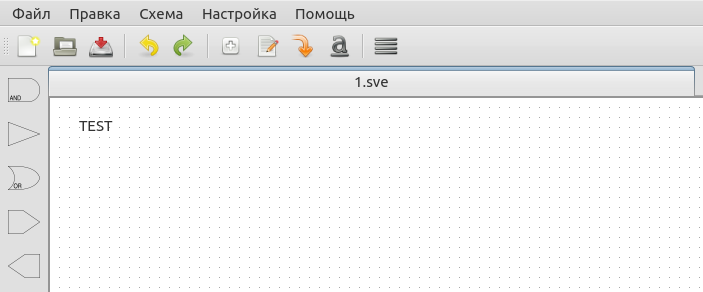
\includegraphics[width=1\textwidth]{gui/test/history-1.png}
  \caption{Созданная схема}
  \label{fig:test-hist-1}
\end{figure}

\begin{figure}[H]
  \centering
  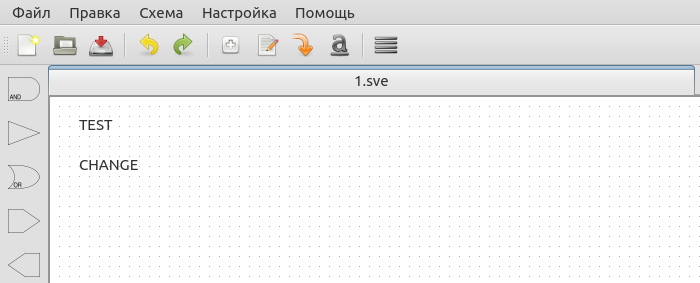
\includegraphics[width=1\textwidth]{gui/test/history-1-change.png}
  \caption{Схема со внесенными изменениями}
  \label{fig:test-hist-1-change}
\end{figure}

\begin{figure}[H]
  \centering
  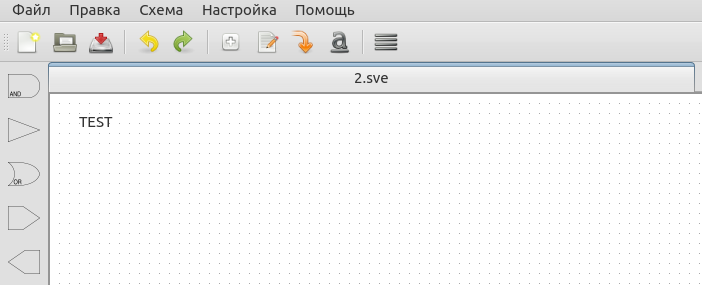
\includegraphics[width=1\textwidth]{gui/test/history-2.png}
  \caption{Схема после отмены изменений}
  \label{fig:test-hist-2}
\end{figure}

Сравнение исходного и измененного файлов:
\begin{lstlisting}
diff -s 1.sve 1-change.sve
\end{lstlisting}

Файлы различаются одной добавленной строкой:
\begin{lstlisting}
4d3
<  <label x="30" id="1400409971081" y="60" text="CHANGE"/>
\end{lstlisting}

Сравнение файлов после отмены изменений:
\begin{lstlisting}
diff -s 1.sve 2.sve
\end{lstlisting}

Файлы идентичны:
\begin{lstlisting}
Files 1.sve and 2.sve are identical
\end{lstlisting}

Очевидно, процесс отмены изменений протекал корректно, сохраняя структуру и содержимое документа.

\subsection{Экспорт схемы в графическом формате}
\textbf{Исходные данные:}
\begin{figure}[H]
  \centering
  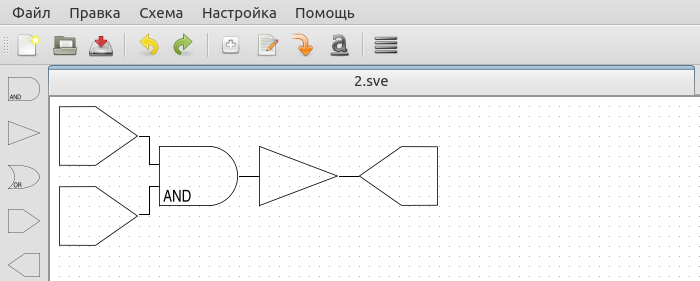
\includegraphics[width=1\textwidth]{gui/test/export-1.png}
  \caption{Экспортируемая схема}
  \label{fig:test-export-1}
\end{figure}

\textbf{Механизм тестирования:}
\begin{enumerate}
  \item Экспортировать схему в формате изображения.
  \item Сравнить полученное изображение с отображаемым в программе.
\end{enumerate}

\textbf{Результат:}
\begin{figure}[H]
  \centering
  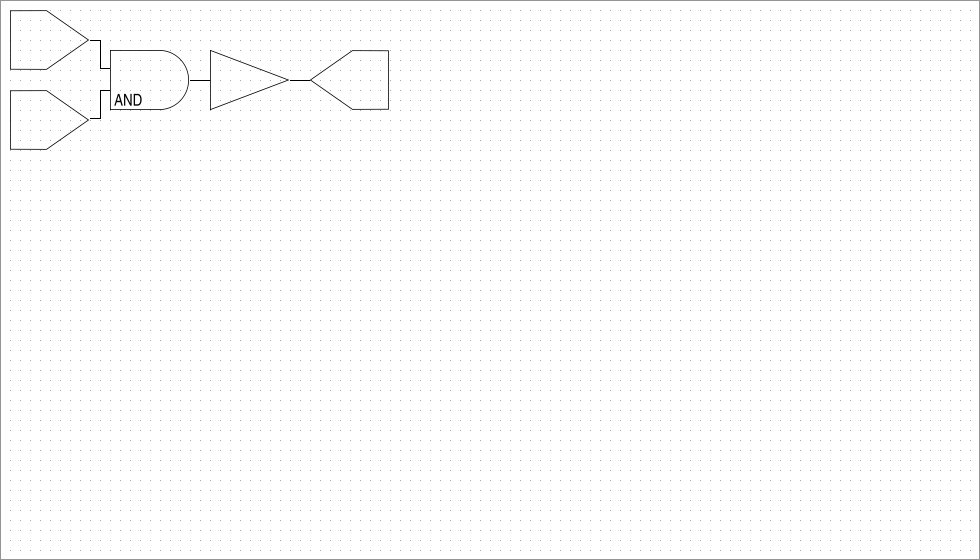
\includegraphics[width=1\textwidth]{gui/test/export-2.png}
  \caption{Экспортированное изображение}
  \label{fig:test-export-2}
\end{figure}

Сравнение рисунков \ref{fig:test-export-1} и \ref{fig:test-export-2} показало, что процесс экспорта схемы в графическом формате работает корректно.

\subsection{Получение программного описания}
\textbf{Исходные данные:}
\begin{figure}[H]
  \centering
  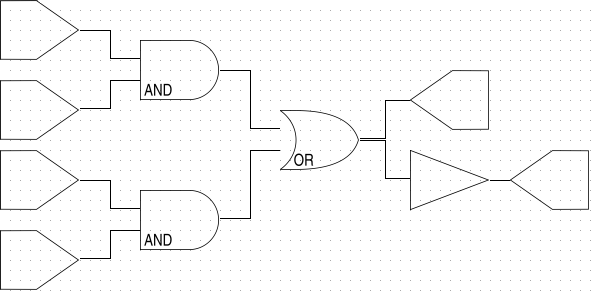
\includegraphics[width=0.6\textwidth]{gui/test/source.png}
  \caption{Проверяемая схема}
\end{figure}

\textbf{Механизм тестирования:}
\begin{enumerate}
  \item Получить программное описание системы.
  \item Проверить корректность синтаксиса.
  \item Скомпилировать систему.
  \item Запустить полученную систему.
\end{enumerate}

Шаги 2 -- 4 выполнялись с использованием утилиты GHDL, назначение которой описано в пункте \ref{sec:software-structure-components}.\\

\textbf{Результат:}

Полученное программное описание:
\begin{lstlisting}
-- SVE direct export

entity and_gate is
port (
	IN1 : in BIT;
	IN2 : in BIT;
	OUT1 : out BIT);
end entity and_gate;

architecture functional of and_gate is
begin
OUT1 <= IN1 and IN2;
end architecture functional;

entity or_gate is
port (
	IN1 : in BIT;
	IN2 : in BIT;
	OUT1 : out BIT);
end entity or_gate;

architecture functional of or_gate is
begin
OUT1 <= IN1 or IN2;
end architecture functional;

entity not_gate is
port (
	IN1 : in BIT;
	OUT1 : out BIT);
end entity not_gate;

architecture functional of not_gate is
begin
OUT1 <= not IN1;
end architecture functional;

-- SVE entity
entity sve is
port (
	SVEIN1 : in BIT;
	SVEIN2 : in BIT;
	SVEIN3 : in BIT;
	SVEIN4 : in BIT;
	SVEOUT1 : out BIT;
	SVEOUT2 : out BIT);
end entity sve;

architecture structure of sve is
component and_gate is
port (
	IN1 : in BIT;
	IN2 : in BIT;
	OUT1 : out BIT);
end component and_gate;

component or_gate is
port (
	IN1 : in BIT;
	IN2 : in BIT;
	OUT1 : out BIT);
end component or_gate;

component not_gate is
port (
	IN1 : in BIT;
	OUT1 : out BIT);
end component not_gate;

signal SVESIG1: BIT;
signal SVESIG2: BIT;
signal SVESIG3: BIT;
signal SVESIG4: BIT;
signal SVESIG5: BIT;
signal SVESIG6: BIT;
signal SVESIG7: BIT;
signal SVESIG8: BIT;
signal SVESIG9: BIT;

begin
	SVESIG1 <= SVEIN1;
	SVESIG2 <= SVEIN2;
	SVESIG3 <= SVEIN3;
	SVEOUT1 <= SVESIG6;
	SVEOUT2 <= SVESIG8;
	SVESIG9 <= SVEIN4;
	SVESIG7 <= SVESIG6;
	SVENODE4 : and_gate port map (SVESIG1, SVESIG9, SVESIG4);
	SVENODE5 : and_gate port map (SVESIG2, SVESIG3, SVESIG5);
	SVENODE6 : or_gate port map (SVESIG4, SVESIG5, SVESIG6);
	SVENODE8 : not_gate port map (SVESIG7, SVESIG8);
end architecture structure;
\end{lstlisting}

Данный программный код был сохранен в файл sve.vhdl.

Проверка корректности синтаксиса:
\begin{lstlisting}
ghdl -s sve.vhdl
\end{lstlisting}

Выполнение команды не привело к выводу сообщений об ошибках, значит, полученное программное описание синтаксически верно.

Проверка компилируемости системы:
\begin{lstlisting}
ghdl -a sve.vhdl
\end{lstlisting}

Указанная команда была первым шагом компиляции и выполняет анализ системы.
Выполнение ее не привело к выводу сообщений об ошибках, а в результате работы были созданы файлы \textbf{work-obj93.cf} и \textbf{sve.o}.

Первый файл~--- компонентный файл, описывающий структуру конечной системы, второй~--- объектный файл системы.

Следующим шагом было построение системы:
\begin{lstlisting}
ghdl -e sve
\end{lstlisting}

Ошибок также не возникло, был создан файл \textbf{sve}~--- исполняемый файл системы.

Проверка запуска:
\begin{lstlisting}
ghdl -r sve
\end{lstlisting}

Процесс завершился корректно, без сообщений об ошибках.

Можно сделать вывод, что получаемые в результате работы системы программные описания синтаксически корректны и компилируемы.